\section{Непрерывное и дискретное преобразование Фурье}
Для начала ура ура опять старая добрая волна:

\begin{equation}
    \Pi(t) = 
    \begin{cases}
        1, |t| \leq \frac{1}{2} \\
        0, |t| > \frac{1}{2}
    \end{cases}
\end{equation}

Я если честно больше не хочу делать ее график, потому что мы его 100 раз видели, он такой типо - 

\begin{equation}
    \_\_\_\_\_|^{-}|\_\_\_\_\_
\end{equation}

Дааа, красиво.

Ладно, вот настоящий:

\begin{figure}[ht]
    \centering
    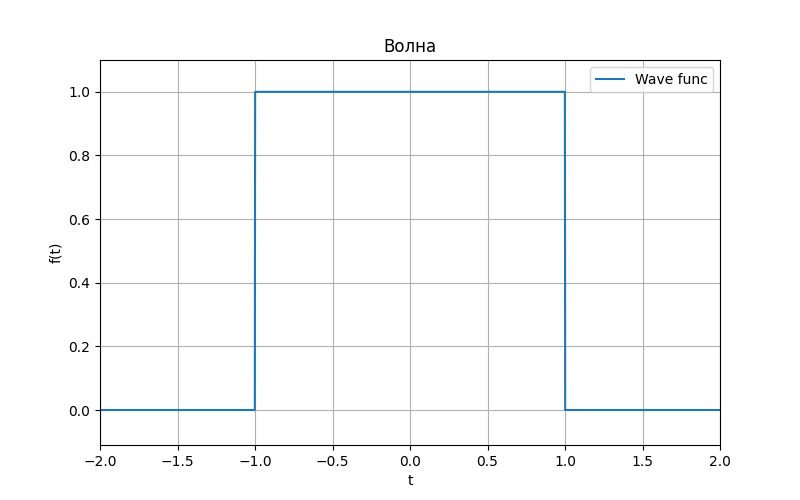
\includegraphics[width=1\textwidth]{/Users/nikolajprovorov/Yandex.Disk-368690@edu.itmo.ru.localized/Lab_5_FURRY/plots/1000_20/wave_func.png}
    \caption{График волны}
\end{figure}

\clearpage

\subsection{Истнинный Фурье - образ.}

Ну придумали, аналитически, да где это видано. А у меня в работе и видано:

\begin{align}
    \hat{\Pi}(\nu) = \int\limits_{-\infty}^{+\infty} \Pi(t) e^{-2\pi i\nu t} dt = \int\limits_{-\frac{1}{2}}^{+\frac{1}{2}} e^{-2\pi i\nu t} dt = \frac{e^{\pi i\nu} - e^{\pi i\nu}}{-2\pi i\nu} = \frac{\sin(\pi\nu)}{\pi\nu} = sinc(\pi \nu)
\end{align}

Ну и график, без него никуда:

\begin{figure}[ht]
    \centering
    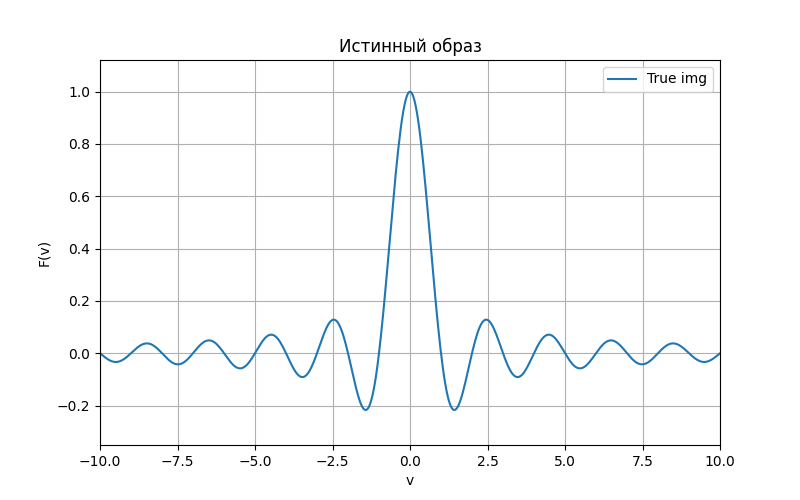
\includegraphics[width=1\textwidth]{/Users/nikolajprovorov/Yandex.Disk-368690@edu.itmo.ru.localized/Lab_5_FURRY/plots/1000_20/true_image.png}
    \caption{График истинного Фурье - образа}
\end{figure}

\clearpage

\subsection{Численное интегрирование.}

Ну, для начала надо воспользоваться численным методом интегрирования. Ну, так как оно численно, а то есть не по бесконечному промежутку, то возьмем первый отрезок $[-20; 20]$.

\begin{figure}[ht]
    \centering
    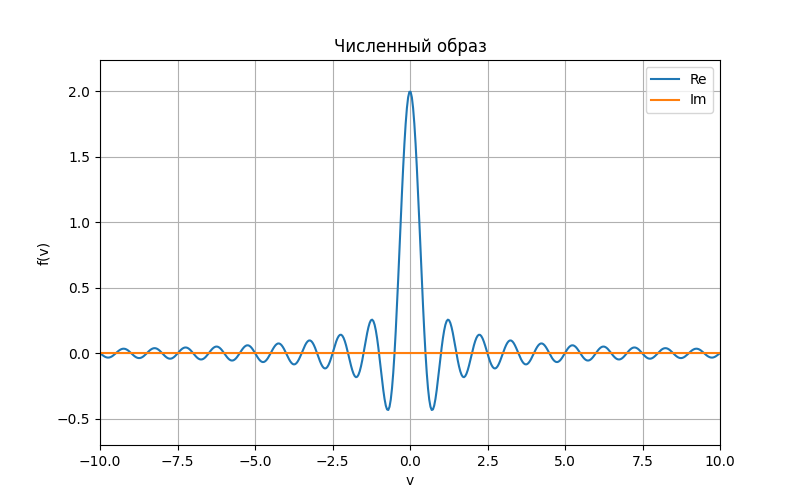
\includegraphics[width=1\textwidth]{/Users/nikolajprovorov/Yandex.Disk-368690@edu.itmo.ru.localized/Lab_5_FURRY/plots/1000_20/num_image.png}
    \caption{График численного Фурье - образа}
\end{figure}

Они совпадают, можно идти дальше

\subsection{Восстановление волны.}

Посмотрим насколько точно удастся восстановить волну по ее численно-интегрированному Фурье - образу. 

\begin{figure}[ht]
    \centering
    \includegraphics[width=1\textwidth]{/Users/nikolajprovorov/Yandex.Disk-368690@edu.itmo.ru.localized/Lab_5_FURRY/plots/1000_20/cmp_restored.png}
    \caption{Сравнение восстановленной волны и исходной}
\end{figure}

Довольно точно.

\clearpage

\subsubsection{Влияние величины шага и размера промежутка}

Рассмотрим другой промежуток интегрирования: 50.

\begin{figure}[ht]
    \centering
    \includegraphics[width=1\textwidth]{/Users/nikolajprovorov/Yandex.Disk-368690@edu.itmo.ru.localized/Lab_5_FURRY/plots/1000_50/cmp_restored.png}
    \caption{Сравнение восстановленной волны и исходной}
\end{figure}

Еще посмотрим на влияние шага интегрирования: вместо 1000 возьмем 5000.

\clearpage

\begin{figure}[ht]
    \centering
    \includegraphics[width=1\textwidth]{/Users/nikolajprovorov/Yandex.Disk-368690@edu.itmo.ru.localized/Lab_5_FURRY/plots/5000_50/cmp_restored.png}
    \caption{Сравнение восстановленной волны и исходной}
\end{figure}

После этого можно немного порассуждать. Мы можем заметить, что при увеличении промежутка интегрирования функция восстанавливается лучше, что немного странно. Что касается шага интегрирования, то при увеличении шага восстановление волны становится лучше, что вполне логично.

\clearpage

\subsection{Дискретное преобразование Фурье (использование DFT)}

Для начала посмотрим как считается FFT в бибилиотеке numpy

\begin{equation}
    A(k) = \sum_{m = 0}^{n - 1}a(m)e^{2\pi i\frac{mk}{n}}
\end{equation}

А обратное:

\begin{equation}
    a(m) = \frac{1}{n}\sum_{k = 0}^{n - 1}A(k)e^{2\pi i\frac{mk}{n}}
\end{equation}

К унитарному приведено параметром, так что все ок.

\subsubsection{Найденный образ и восстановленная функция.}

Посмотрим на образ и восстановленную функцию.

\begin{figure}[ht]
    \centering
    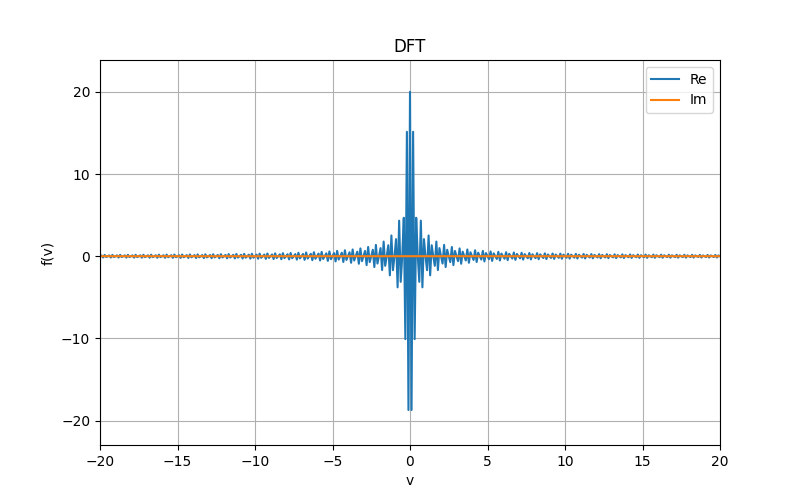
\includegraphics[width=0.8\textwidth]{/Users/nikolajprovorov/Yandex.Disk-368690@edu.itmo.ru.localized/Lab_5_FURRY/plots/fft_10000/dft_image.png}
    \caption{Образ функции}
\end{figure}

\clearpage

\begin{figure}[ht]
    \centering
    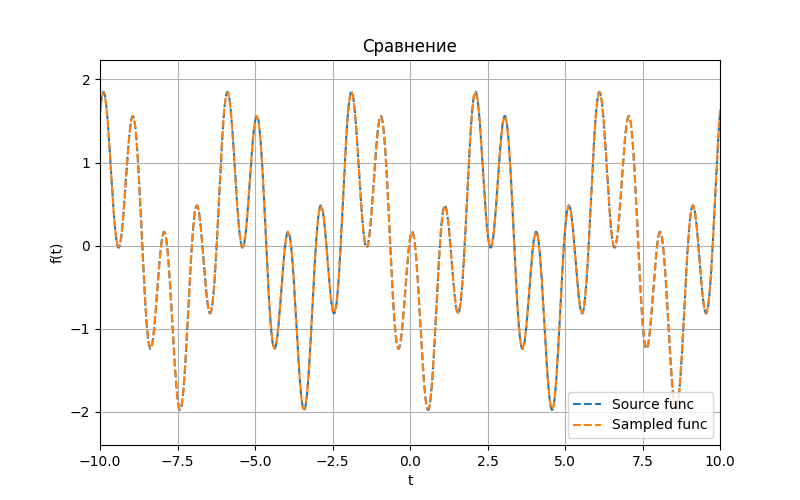
\includegraphics[width=0.8\textwidth]{/Users/nikolajprovorov/Yandex.Disk-368690@edu.itmo.ru.localized/Lab_5_FURRY/plots/fft_10000/cmp_func.png}
    \caption{Сравнение восстановленной функции и исходной}
\end{figure}

Выглядит очень прикольно, да и время тратится значительно меньше. КРУТО!

\subsection{Приближение непрерывного с помощью DFT}

Что же было не так в прошлом пункте? Вам, как, я думаю, и мне, не понравился образ, полученный в результате DFT. Он явно не похож на истинный. Но что же нам делать?

Давайте попробуем дискретизировать преобразование Фурье. Для этого введем 2 параметра: $t_d = m\triangle t + t_0, \upsilon_d=k\triangle \upsilon$. Они нужны для того чтобы ввести дискретное время и частоту. Посмотрим что получится:

\begin{equation}
    \hat{f}(\upsilon) = \sum_{m = 0}^{N - 1}f(t_d)e^{-2\pi i\upsilon} \triangle t = \triangle t e^{-2\pi i\upsilon _d t_0} F(t_d),~\text{где}~ F(t_d) - \text{DFT образ}
\end{equation}

Получается, что для получания образа надо умножить на $ \triangle t e^{-2\pi i\upsilon _d t_0} $ DFT образ. Посмотрим на результат:

\begin{figure}
    \centering
    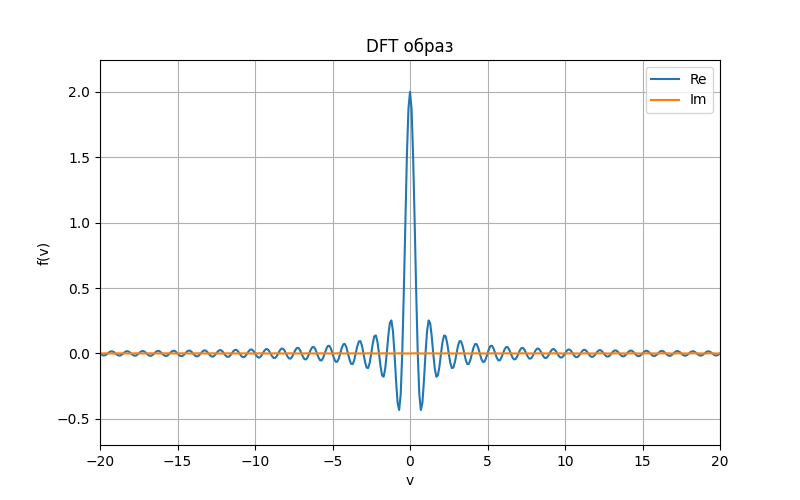
\includegraphics[width=0.8\textwidth]{/Users/nikolajprovorov/Yandex.Disk-368690@edu.itmo.ru.localized/Lab_5_FURRY/plots/fft_10000/dft_cont_image.png}
    \caption{Истинный образ функции с помощью DFT}
\end{figure}

А восстановленная функция соответственно (рис. 10.):

\begin{figure}
    \centering
    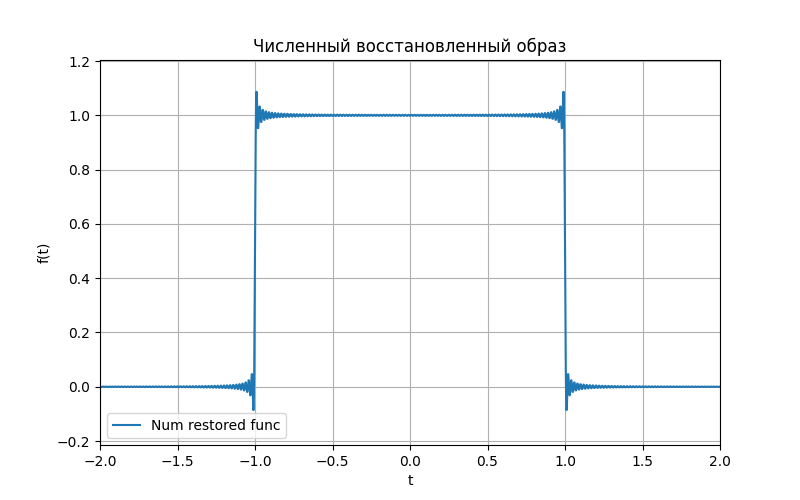
\includegraphics[width=0.8\textwidth]{/Users/nikolajprovorov/Yandex.Disk-368690@edu.itmo.ru.localized/Lab_5_FURRY/plots/fft_10000/num_restored.png}
    \caption{Восстановленная функция}
\end{figure}

Получается, все получилось.

\clearpage

\subsection{Влияние шага и размера промежутка}